\section{ХОД РАБОТЫ}

\subsection{Текст задания}

Необходимо необходимо выполнить следующее:
написать программу на основе предыдущей лабораторной работы №7.

Во всех вариантах заданий требуется синхронизировать потоки с помощью
одного из нижеприведенных методов синхронизации:

\begin{itemize}
\item критическая секция;
\item mutex;
\item событие;
\item семафор.
\end{itemize}

\subsection{Исходные данные}

На рисунке~\ref{lst:complex_h_code} представлено содержимое наиболее
важных заголовочных файлов, реализованных в предыдущих лабораторных работах.

\begin{lstlisting}[caption=Исходный код заголовочного файла complex.h,label=lst:complex_h_code]
struct Complex {
    double re;
    double im;
};

void writeComplex(char *fname,
                  struct Complex *complex,
                  int count);

struct Complex input_complex();
\end{lstlisting}

Функции, приведенные на рисунке~\ref{lst:complex_h_code},
были использованы при выполнении лабораторной работы №8.

\subsection{Теоретические сведения}
\label{ssec:therory}

\paragraph{}
Для синхронизации задач в разрабатываемом приложении будет использоваться 
семафор, как наиболее универсальное средство синхронизации.
Поэтому считаем уместным привести описание работы с семафорами в
ОС семейства Windows.

\paragraph{}
\textit{Семафор} --- объект, ограничивающий количество потоков, 
которые могут войти в заданный участок кода. 

\paragraph{}
Для создания семафора в ОС Windows задача должна вызвать функцию CreateSemaphore,
прототип которой приведен на рисунке~\ref{lst:create_semaphore}.

\begin{lstlisting}[caption=Прототип функции создания семафора,
  label=lst:create_semaphore]
HANDLE CreateSemaphore (
  LPSECURITY_ATTRIBUTES lpSemaphoreAttributes,
  LONG lInitialCount, 
  LONG lMaximumCount, 
  LPCTSTR  lpName);
\end{lstlisting}

Параметр \textit{lpSemaphoreAttributes} описывает значения атрибутов защиты,
параметры \textit{lInitialCount} и \textit{lMaximumCount} обозначают начальное и 
максимальное значения счетчика, связанного с создаваемым семафором.
Параметр \textit{lpName} представляет собой адрес строки с именем семафора.

\paragraph{}
Существующий семафор можно открыть функцией OpenSemaphore, 
прототип которой приведен на рисунке~\ref{lst:open_semaphore}.

\begin{lstlisting}[caption=Прототип функции открытия семафора,
  label=lst:open_semaphore]
HANDLE OpenSemaphore (
  DWORD   fdwAccess,
  BOOL    fInherit, 
  LPCTSTR lpszSemaphoreName);
\end{lstlisting}

Параметр \textit{fdwAccess} определяет требуемый уровень доступа к семафору.
Параметр \textit{fInherit} определяет возможность наследования полученного идентфикатора.
Параметр \textit{lpszSemaphoreName} представляет собой адрес символьной строки,
содержащей имя семафора.

Если семафор открыт успешно, функция \textit{OpenSemaphore} возвращает его идентификатор.
При ошибке возвращается значение NULL.

\paragraph{}
Для увеличения значения счетчика семафора приложение должно использовать
функцию ReleaseSemaphore, прототип которой приведен на рисунке~\ref{lst:release_semaphore}.

\begin{lstlisting}[caption=Прототип функции увеличения счетчика семафора,
  label=lst:release_semaphore]
BOOL ReleaseSemaphore (
  HANDLE hSemaphore,
  LONG cReleaseCount,
  LPLONG lplPreviousCount);
\end{lstlisting}

Параметр \textit{hSemaphore} представляет собой идентификатор семафора,
\textit{cReleaseCount} --- значение инкремента, \textit{lplPreviousCount} ---
адрес переменной для записи предыдущего значения счетчика семафора.

\paragraph{}
В программном интерфейсе операционной системы Microsoft Windows NT нет фукнции,
специально предназначенной для уменьшения значения счетчика семафора.
Этот счетчик уменьшается, когда задача вызывает функции ожидания, 
такие как \textit{WaitForSingleObject()} или \textit{WaitForMultipleObject()}.
Если задача вызывает несколько раз функцию ожидания для одного и того же семафора,
содержимое его счетчика каждый раз будет уменьшаться.

\subsection{Особенности разработанной программы}
\label{ssec:program_description}

Разработанная программа записывает в файл вводимые пользователем комплексные числа. 

Главный поток программы предлагает пользователю ввести выбранное количество
комплексных чисел.
После успешного ввода в программе порождается новый поток, 
записывающий введенные данные в файл.
В это время пользователь имеет возможность повторить ввод данных, 
которые сохраняются в динамически выделяемой памяти независимо от других данных,
а затем записываются новым потоком записи.

Для синхронизации доступа к файлу между дочерними потоками используется семафор.
В качестве разделяемого ресурса выступает файл, в которые производится запись.

Особенностью разработанной программы является тот факт, что 
семафор не является глобальной переменной, а передается в качестве параметра 
функции, вызываемой в дочернем потоке.

Для взаимодействия с дочерним процессом используется структура,
представленная на рисунке~\ref{lst:complexes}. 

\begin{lstlisting}[caption=Структура Complexes,
  label=lst:complexes]
struct Complexes {
	HANDLE semaphore;
	int count;
	struct Complex* complexes;
};
\end{lstlisting}

Поле \textit{semaphore} представляет собой дескриптор семафора,
\textit{count} --- количество комплексных чисел, которые требуется записать,
\textit{complexes} --- динамический массив, содержащий комплексные числа, ожидающие записи.

После успешной записи происходит освобождение памяти, выделенной 
для хранения структуры complexes.

Главное окно программы показано на рисунке~\ref{fig:main_screen}.

\begin{figure}[htbp]
  \centering
  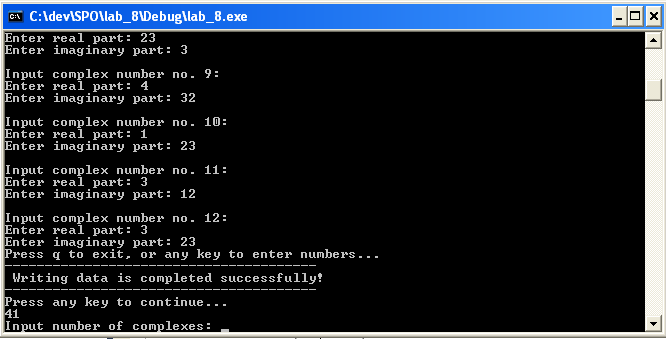
\includegraphics[width=150mm,height=80mm]{img/main_screen}
  \caption{Главное окно программы}\label{fig:main_screen}
\end{figure}


Исходный текст разработанной программы расположен в приложении~А.

\newpage